

Use 'closed part of a system'. "We close a system, or we keep an open approach"

The part of the system we have closed can still be complicated. 

In this chapter we use the idea of a closing a system, to help us think about the different systems modelled using machine learning and other mathematical tools. We start by showing that we can close systems do exist in the form of games, experiments in physics and within data sets themselves. Within these closed systems, we can define good practices for modelling them. Indeed, many of the techniques taught on mathematical modelling courses constitute exactly these practices. 

These examples also raise a larger question: what do these closed systems tell us about the real-life, complex, open world? Reality is not a board game or a computer game. A controlled experiment at the atomic or sub-atomic level tells us nothing about our social interactions at work and home. Data about shots in football or the box office success of films is not the same as an actual game of football or a Hollywood movie. The map of an area is not the territory itself.

We will thus broadly separate the systems we model in to approaches two categories: {\it closed systems}, where we have a set of well-defined modelling tools to provide answers about that system, and {\it open systems}, where we have to make a (oftentimes subjective) decision how to close the system in order to apply our tools. The set of closed systems is large, and we will meet many examples during this course, but the set of open systems is even larger and encompasses the biggest challenges 


\section{Board and computer games}

Inside chess there are rules (e.g. white plays first; pawns can move one step or two steps forward on their first move and only one thereafter; the queen can move both backward and forward as well as diagonally and so on). These rules define how we are allowed to act, to play, in every circumstance. As a result, we can write an algorithm which, when shown a chess board with a particular arrangement of pieces, can list all the valid moves. 

In the previous chapter, we stated that the only time we can say we have a complete model of a system is when our model is the the system itself. For chess this is possible. And it is this sense, we say the game of chess is closed. We can capture everything about the game in a model by saying which rules are valid and which are not.

Once we have closed the game in this way, we can also define a mathematical problem within which we calculate, for any given arrangement of pieces on the board, which move will give the best chance of winning the game. It is is thus (in theory) possible to solve chess once and forever and provide the optimal move for any arrangement of pieces. 

In practice, it has also proved possible to build a computer that is better at finding the best moves than humans. The first algorithm that could beat all living humans was Deep Blue. In 1997,

Deep Blue was more closer to a mechanistic model of chess than . 



We can say 

All computer games are closed games. Most, if not all computer games, are played better by a machine learning model than by humans. The exact 



Not all games are completely closed, in the sense that their rules are unambiguous, like those of chess. We will return to this point in chapter \ref{mapterritory} (and also investigate ways in which chess can be made open). For now, we turn our attention to physical, chemical and biological systems. Can some of these be considered as closed?


\section{Physical processes}


Weather models.


\section{Data}

In isolation, a data set constitutes a closed system. This is because data is by its nature an array of 1s and 0s, stored inside a computer (or expressed in a way that would allow it to be stored inside a computer). It is usually possible to create a model of a data set which is simpler than the data itself, in the sense that we can compress the data. For example, when we create a zip file we make the file smaller, but because we can recover the original data again, we know that we have 

Another way of reducing data is to fit a model to it. 


But the data is not the system itself,  




In machine learning, a distinction is made between training and test data. The training data is used to create and fit the model. The test data is then used to measure model performance on unseen data. The reason for taking this approach is to test the degree to which the model is overfit to the specific data on which it was trained. 

We can see the training data as a closed system. When we fit the model to it we are representing that data (and that data only) in the form of a model. When we introduce the test data, we open up the model to a new part of the world on which the model is tested. We test the degree to which the model can deal with that more open part of the world.

While the training/test split reveals the closed nature of the training set, we should remember that the combined training/test set is also closed. Usually, the training and test sets will be randomly sampled from a larger data set. For example, if we have a data set of 1000 shots from football games, 900 might be randomly chosen from these for training and 100 used for testing. Thus, the test/training divide is just an arbitrary division of a closed system in to two parts. 


No matter how much training and testing we have done of a model, we still have to justify how it relates to the open system which constitutes the real world. For example, if we were to apply the expected goals model to a season of football in the same league on which the model is fit, would we consider it a reasonable model? In this case, we probably would.

But would the model still be reasonable ten years from now, 
womens football, youth football, At some point it stops being a reasonable model. 

Model error. 



\cite{waldrop2022beyond}



\section{A case study: Hollywood film data}



The film data set is not the same thing as the Hollywood film industry. 



When we analyse the data set and explain our results to others, we take a specific view. 


- Who created the data set and why?

- Is this just how things are 

Emphasise fact can't capture the entire nature of the system. Depdening on how good and careful cautious you are you are capturing some element.

\section{The two modelling cultures}

\label{sec:twocultures}

In a article published in 2001, Leo Breiman described two cultures in modelling. The first culture assumes that data is generated by a specific {\it mechanism}, while the other concerns itself solely with {\it data}, and treats the mechanism as unknown. We already drew figures illustrating these approaches: figure \ref{fig:Mechanism} illustrates the construction of a mechanistic model, while figure \ref{fig:SupervisedLearning} illustrates a supervised learning approach, where patterns in the data are learnt by the model. The models we created of goals in football --- one based on the geometry of shooting (mechanism), the other based on use of all available data (data-driven) --- illustrate the different approaches. As do the framing of the question ``Can we identifying a Hollywood blockbuster?'' in terms of pure prediction (what the data tells us) or in terms of the role gender has played in Hollywood (mechanism).

Even when we are dealing with closed system, it is not always clear whether a data-driven or mechanistic approach is most appropriate. Breiman's article challenged the statisticians of the time, in asserting that the mechanistic approach ``led to irrelevant theory, questionable conclusions, and has kept statisticians from working on a large range of interesting current problems´´. He showed how random forest models, 

The success of Alpha Zero in creating winning strategies for Go and Chess without any prior information is evidence in favour of the data-driven approach for these and many other game applications. However, some even relatively simple games have remained 


In image analysis, the data-driven approach has proven most successful. 



Attention is all you need...


Any problem 


As Melanie Mitchell writes, “even the most general version, AlphaZero, is not a single system that learned to play Go, chess, and shogi. Each game has its own separate convolutional neural network that must be trained from scratch for its particular game.” 


In conclusion, we note that even within the confines of closed problems there remains debate over whether mechanistic or data-driven approaches are best suited to particular cases. It is though, on balance, it is fair to say that data-driven approaches are now more important for applications involving predictions in closed games and data sets. Many closed problems can be solved without specifying features. For others key features of the problem can be identified, and these (along with some other features that did not appear important in a mechanistic model) can be used to produce highly effective models using neural networks, random forests and other machine learning approaches. 

\section{The map is not the territory}

All mathematical modellers occasionally use language which confuses models for reality. 


\subsection{All models are...}

An often used quote in the context of the relationship between models and reality is George Box aphorism: ``All models are wrong but some are useful''

Box wrote that ``the question you need to ask is not "Is the model true?" (it never is) but "Is the model good enough for this particular application?"'' 

This phrase could be a useful tool for explaining something similar to the map is not the territory idea, but it is not as . To see these, let's look more closely at the use of the words `true´ and `useful'. Imagine you have invited a friend, called Deirdre, for dinner and she have said she will come. You know that Deirdre is usually reliable and often comes to your house. Now imagine that another friend, George, tells you that is isn't true that Deirdre will come, then how you would react? Most of us would be surprised, we would ask George what he knows that we don't. But George doesn't have any extra information, he simply replies that you cannot know for sure that Deirdre will come over, so it isn't true. She might start to feel unwell, remember she has other plans or get hit by a bus on the way to your house, he says. It might be {\it useful} to assume she will come, he says, but it isn't {\it true}!

George is not being particularly helpful here. He is creating a distinction between the words true and useful that are at odds with how we use them. Imagine he did that with every statement you make: `it isn't true   `it isn't true that the sun will come up tomorrow´... 


George Box aphorism isn't particularly true or useful, since it builds on a distinction we seldom make in real life. It encourages a view of modelling that is unhelpfully sceptical, while failing to acknowledge the real challenges. A model should not be judged not primarily in terms of whether it is useful in the sense of `good enough for application', but also in terms of the assumptions it makes, how it relates to previous models, the view it constructs of the world and the consequences for those using it for taking that view.  

The map and territory aphorism allows us to get closer to the essence of what we do when we create a model. Consider, for example, visualisations of population, wealth, on a world map in figure \ref{fig:WealthMap}. The wealth map is distorted from geographic reality, but it captures another form of reality: the inequality in financial wealth across the planet.

\begin{figure}[t]
\centering
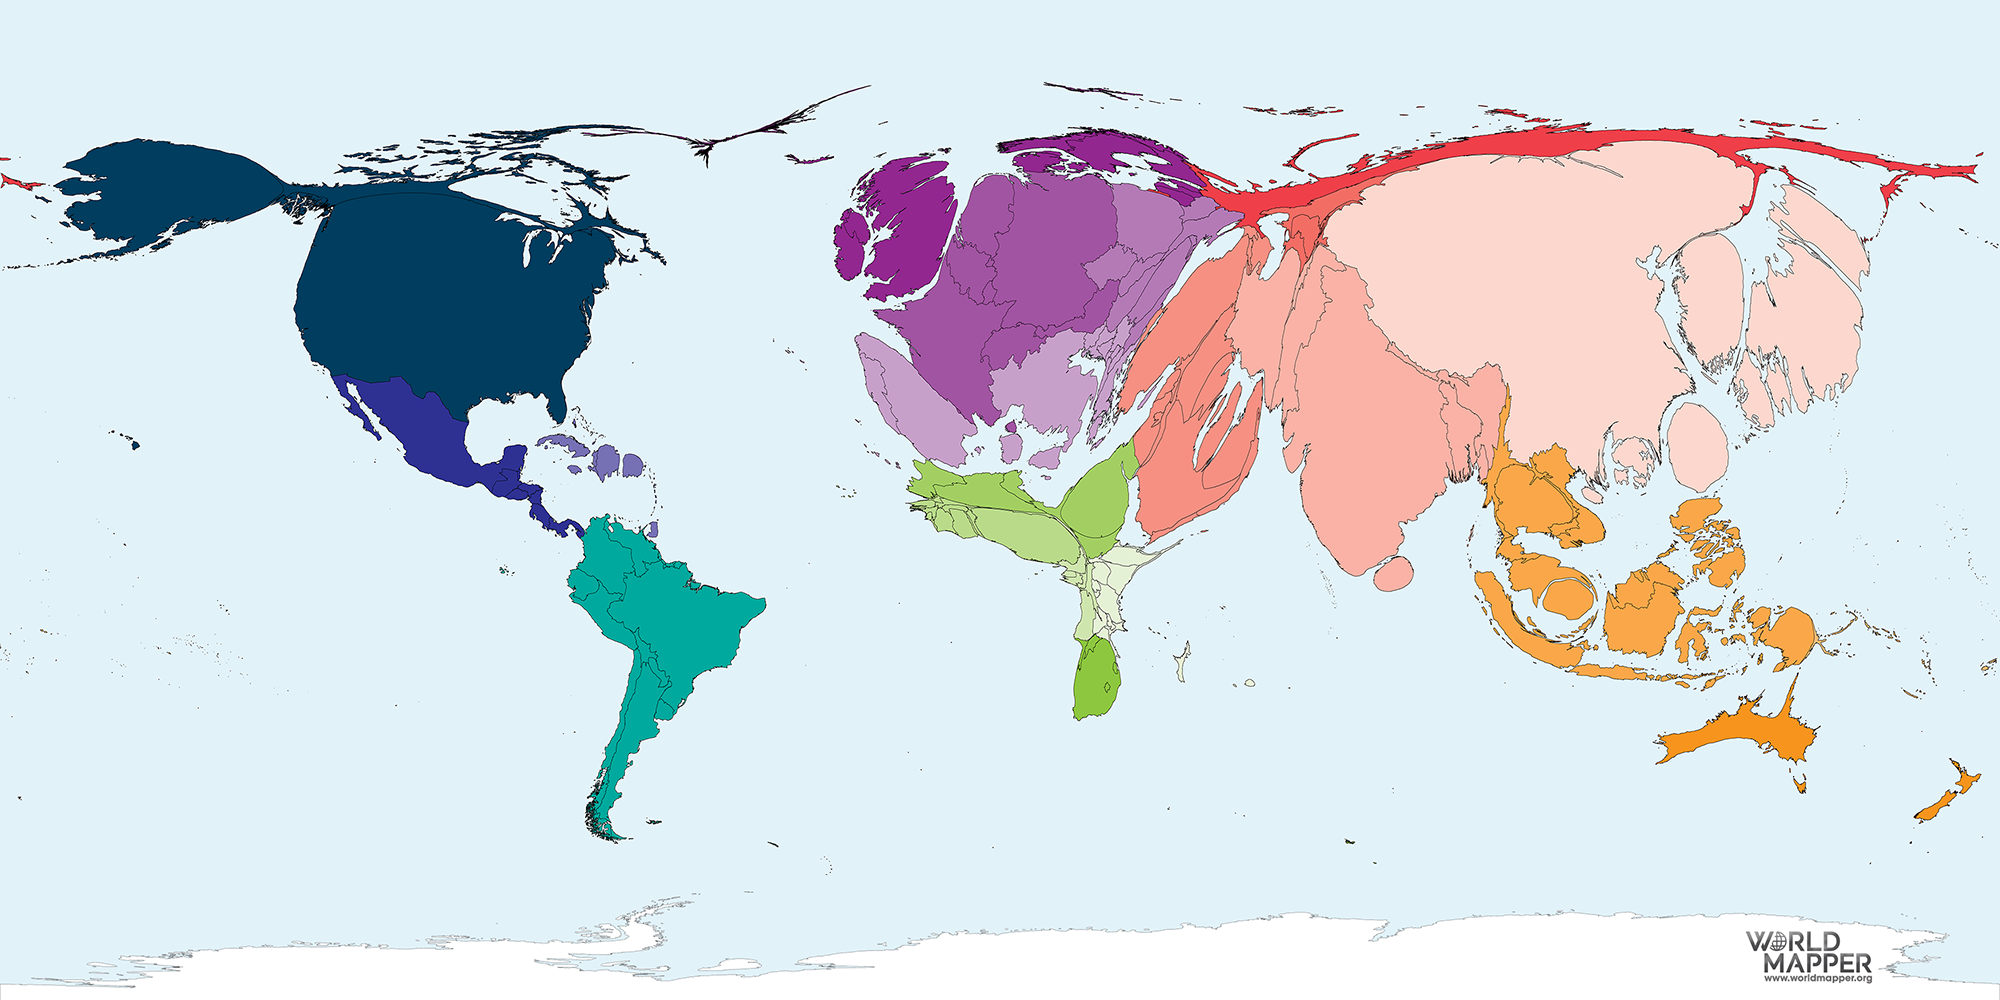
\includegraphics[width=10cm]{Figures/Closed/WealthMap}
\centering
\caption{An illustration of the supervised learning problem.   \label{fig:WealthMap}}
\end{figure}

The question is not whether a model is true or not, but to understand that, like there are many different ways of making maps, there are also many different ways of drawing a map and creating models. Each of them can be a useful (and, in everyday usage of the word, true) guide to the world around us. In the next chapter, we will look at ways of approaching modelling complex, open systems which accounts for this observtaion. 


\subsection{A picture is not enough}

After Deepmind's success with Alpha Zero, one of the research leads on that project David Silver, together with Richard Sutton (a pioneer of reinforcement learning) and other researchers, published an  article claiming that the method they used could be used to explain human abilities, including “knowledge, learning, perception, social intelligence, language, generalisation and imitation”. They even suggested that reinforcement learning could ‘constitute a solution to artificial general intelligence’, the problem of creating a truly human-like machine. Silver acknowledged, in an interview with Wired, that while his hypothesis ‘flies in the face of how a lot of people view AI’, he holds fast to the belief that there is ‘one very clear and simple way to think about all of intelligence … and all of these other things will emerge from that process.’

\begin{figure}[t]
\centering
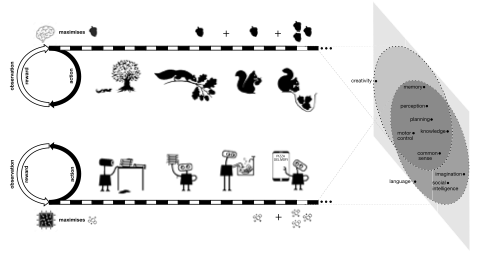
\includegraphics[width=10cm]{Figures/Closed/Squirrel.png}
\centering
\caption{A cartoon representation of a squirrel and a robot, reproduced from Silver et al 2021 \cite{silver2021reward} \label{fig:Squirrel}}
\end{figure}


The argument put forward to support Silver and his colleagues claim uses figure \ref{fig:Squirrel}. They argue that both the robot and the squirrel are examples of reinforcement learning: the squirrel ‘learns’ that getting acorns pays off and evolves more advanced strategies for collecting them and the cleaning robot ‘learns’ that it pays to tidy up and ‘evolves’ to clean its environment.

This cartoon is certainly one valid way of comparing a robot and a squirrel, and biologists sometimes use this paradigm – known as optimal foraging – to understand squirrels’ strategic foraging decisions.  But biologists also know that this paradigm is far from the only way to describe a squirrel. When scientists study animals, they look at: their place in the evolutionary tree; how they evolved to forage on land or at sea; they study physiology and neurology; the viruses and bacteria living inside them; visual and olfactory systems; the chemical processes involved in digesting food; how animal behaviour has been shaped by interactions with humans; and how it is shaped by changing environments and climate change. The ‘squirrel as learning to maximise acorn collection’ is just one of many successful paradigms in biology. 

Figure \ref{fig:Squirrel} creates a visual analogy, mapping a squirrel onto a simulated kitchen robot, by finding one way in which they are similar. Such visual analogies are appealing, but they can also be deceptive, because they deliberately hide complexity. They conceal all the very different ways in which we can look at a squirrel. They hide its complexity. 

Silver and colleagues’ article makes a series of visual analogies. The authors juxtapose five systems: the board game Go (on which reinforcement learning performs well), a robotic agent (in a computational simulation), a physical robot, a squirrel (which they interchange with human behaviour, natural agents, and animals in general) and Artificial General Intelligence (AGI). Their hypothesis is that we can move from Go, to a simulated agent (which they equate to a physical robot), to natural agents, to AGI. As illustrated in figure \ref{fig:ComplexityIncrease}.

\begin{figure}[t]
\centering
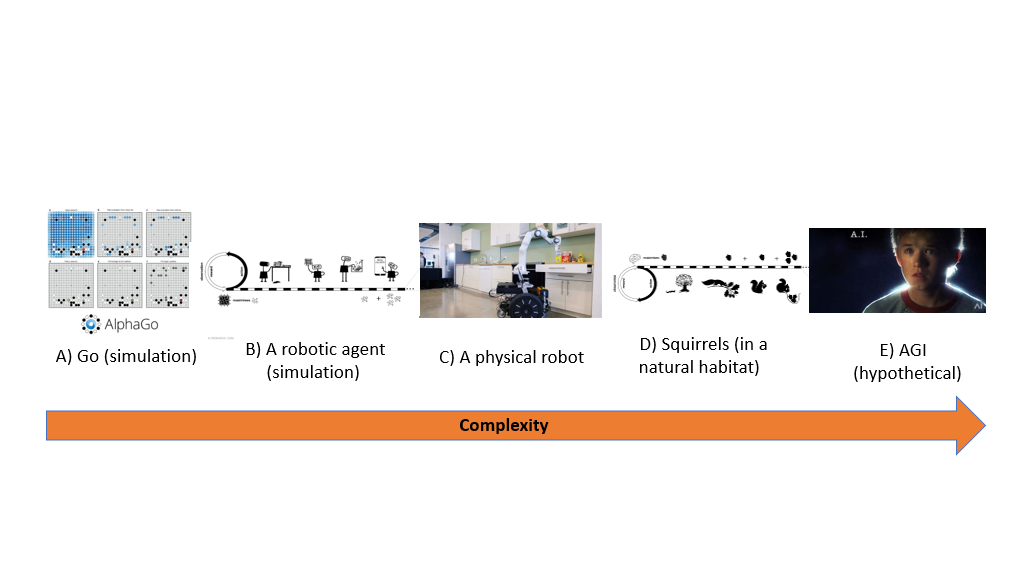
\includegraphics[width=10cm]{Figures/Closed/ComplexityIncrease.png}
\centering
\caption{An illustration of the supervised learning problem.   \label{fig:ComplexityIncrease}}
\end{figure}

Using the approach we have outlined through this chapter we can see the problem of such an argument. Go is a closed game, with well-defined rules and a way of measuring who has won. The cleaning robot simulator is also a closed system. As we discussed in section \ref{sec:twocultures}, it is not currently known whether a problem like this is best solved by 'rewards alone' as proposed by Silver and colleagues (the data-driven approach) or whether a mechanistic model will be needed to build such a robot, even in the closed environment of a computer simulation. 

The important point here, though, is that the jump from a computer simulation to a real-world system means making a move from a closed system to an open system. To claim that a model that works in a computer simulation can be used to tidy living rooms is to confuse the map and the territory.
Current cleaning robots are programmed with additional poop recognition systems, because reinforcement learning can’t teach them that their owners don’t want excrement spread all over the living room floor (spreading dust out before hoovering up is unproblematic, but…). 

Equally, a squirrel is not an Artificial General Intelligence (AGI). There are many different possible models of a human and of a squirrel and there is no way of mapping between the two. We currently lack a clear understanding of what human intelligence is, and the notion of AGI is even more contested and fragmented. There is no clear consensus on how it might be achieved or even if it is possible to build it at all. We will return to this point in chapter \ref{chap:AGI}.




\subsection{Every problem can be opened}




There are ways in which chess can be opened up. For example, consider an older brother playing chess with his little sister. Early in the game, the older sibling might let the younger player retake a move that would have quickly led to her checkmate. They both "break the rules" in order to make a more interesting game. If the younger sister later goes on to place her brother in checkmate, he might remind her that "he let her win." Now, when they report the result to their parents, the outcome is open. The game is no longer just the movement of the pieces itself, but part of a social relation between the players: the older brother still feels he let her win, but he also realises she improved very quickly... Even for him, the game gave rise to an ambiguity. 
